% Template for Cogsci submission with R Markdown

% Stuff changed from original Markdown PLOS Template
\documentclass[10pt, letterpaper]{article}

\usepackage{cogsci}
\usepackage{pslatex}
\usepackage{float}
\usepackage{caption}

% amsmath package, useful for mathematical formulas
\usepackage{amsmath}

% amssymb package, useful for mathematical symbols
\usepackage{amssymb}

% hyperref package, useful for hyperlinks
\usepackage{hyperref}

% graphicx package, useful for including eps and pdf graphics
% include graphics with the command \includegraphics
\usepackage{graphicx}

% Sweave(-like)
\usepackage{fancyvrb}
\DefineVerbatimEnvironment{Sinput}{Verbatim}{fontshape=sl}
\DefineVerbatimEnvironment{Soutput}{Verbatim}{}
\DefineVerbatimEnvironment{Scode}{Verbatim}{fontshape=sl}
\newenvironment{Schunk}{}{}
\DefineVerbatimEnvironment{Code}{Verbatim}{}
\DefineVerbatimEnvironment{CodeInput}{Verbatim}{fontshape=sl}
\DefineVerbatimEnvironment{CodeOutput}{Verbatim}{}
\newenvironment{CodeChunk}{}{}

% cite package, to clean up citations in the main text. Do not remove.
\usepackage{cite}

\usepackage{color}

% Use doublespacing - comment out for single spacing
%\usepackage{setspace}
%\doublespacing


% % Text layout
% \topmargin 0.0cm
% \oddsidemargin 0.5cm
% \evensidemargin 0.5cm
% \textwidth 16cm
% \textheight 21cm

\title{Optimal Models for Resource Allocation in Classroom Teaching}


\author{{\large \bf Larry Liu} \\ \texttt{hrlarry@stanford.edu} \\ Department of Psychology \\ Stanford University \And {\large \bf Michael C. Frank} \\ \texttt{mcfrank@stanford.edu} \\ Department of Psychology \\ Stanford University}

\begin{document}

\maketitle

\begin{abstract}
Teaching is the transmission of knowledge from teacher to student. How
should a school administrator allocate a fixed budget towards increasing
the number of classrooms and increasing student assessment to best
increase student learning? This paper investigates how stochastic models
accounting for the inherent uncertainty in student beliefs and teacher
communication in teacher-student dyads can help school administrators
figure out how to maximize student learning by optimally allocating
resources. We replicate existing results from edu- cation literature
about the effect of class sizes, homogenous ability classrooms, and
assessment on student learning using computer simulation. We also unify
these different determi- nants of student learning into a more holistic
model and report the tradeoffs that committing budget to these design
features presents. We demonstrated that we can create a pareto frontier
for the number of teachers and assessments against a fixed bud- get, and
find an optimal allocation of the budget for increasing student
learning. We also demonstrate how the effectiveness of class sizes and
assessment is contingent upon the learning concept being taught. We
believe that the insights about stu- dent learning in multi-classroom
settings that we've found and can continue to surface are difficult to
surface in real-world studies with human subjects.

\textbf{Keywords:}
Teaching; learning; education; pragmatics; Bayesian modeling; social
cognition
\end{abstract}

Education research has surfaced many insights into policies for
designing schools to improve classroom learning for students. Very
prominently, conventional wisdom makes independent claims that
decreasing class sizes, increasing formative assessments, and increasing
teaching periods \emph{{[}citation needed for last one{]}} improves
student learning outcomes. However, decreasing class sizes and
developing formative assessments compete for a shared resource of money,
while administering formative assessments and teaching lessons compete
for a shared resource of student time. As such, it is important to
understand the diminishing returns for each of these orthogonal design
dimensions in order to find a unified policy that is optimal for student
learning. We call the optimal policy \textbf{optimal school
administration}.

Unfortunately, there exists many barriers to studying optimal school
administration in real-world classrooms. Isolating the effects of a
chosen school design policy would require controlling for student and
teacher differences, and no two classrooms, teachers, and students are
the same. Even if we could control for these sources of random error,
the task of testing hundreds of permutations across multiple policy
dimensions would be time- and cost-prohibitive, along with being
ethically suspect in some extreme cases. As such, the task of
determining optimal school administration lends itself well to computer
modeling.

In this present paper, we turn to stochastic modeling to investigate how
an optimal school administrator might allocate finite resources to
produce maximal information gain. We elect to utilize stochasticity to
build inherent student variability and error on assessments in the real
world into our model. Taken together, this work describes a
first-principles attempt at a framework for understanding resource
allocation in classroom education.

\section{Background}\label{background}

Even when students are motivated to learn, and teachers are motivated to
teach, information transmission in classroom settings are imperfect.
Education in classroom settings has two challenges that we seek to
tackle. First, there exists a problem of \emph{student variability},
where students within the same classroom may have different innate
academic ability as well as upbringings. This means that a lesson that
would be perfect for one child may be less accessible to another child.
Secondly, there exists a problem of \emph{imperfect teacher knowledge}.
Teachers don't have perfect knowledge of each student's personal
knowledge, and this uncertainty potentially results in choices of
teaching exmaples that are not optimal for student learning.

\subsection{Definitions}\label{definitions}

Because our work builds on some fields of research that have different
vocabularies for similar concepts, we first clarify the language and
meanings that will appear in this paper.

\subsubsection{Types of knowledge}\label{types-of-knowledge}

Every student possesses their own malleable \emph{personal knowledge}
about any knowledge concept, which could be facts, skills, beliefs, or
any other type of knowledge. Coloquially, personal knowledge is often
referred to as ability or mastery level, and we use these terms
interchangeably.

Teachers can identify a static \emph{target knowledge} about any
knowledge concept, and a student's personal knowledge can be close to or
far from the target knowledge, representing accuracy or inaccuracy
respectively. The goal of education, therefore, is to adjust the
student's personal knowledge to be as close to the target knowledge as
possible.

Teachers possess beliefs about what their students' personal knowledge
is, which we will call \emph{teacher beliefs}. These may not necessarily
accurately reflect their students' actual personal knowledge.

\subsubsection{Education processes}\label{education-processes}

Assessing, teaching and learning are the three key component processes
of education. \emph{Assessing} involve students providing information to
teachers to \emph{assessments} (e.g.~assignments, quizzes, exams,
classroom participation, etc.) based on their personal knowledge. The
answers provided help teachers update their teacher beliefs.

\emph{Teaching} involves a teacher providing \emph{lessons} to students
to help adjust their students' personal knowledge towards the target
knowledge. The content of the lessons are determined by the teacher
beliefs; in other words, the teacher chooses \emph{teaching examples}
that they believe are most suitable given their students' personal
knowledge.

Finally, \emph{learning} involves a student using the teaching examples
provided by the teacher through teaching to update their own personal
knowledge. Learning itself does not guarantee that a student will update
their personal knowledge to be closer to the target knowledge; the
student must rely on the teacher to pick effective teaching examples for
the updates to be useful.

\subsubsection{Example -- TODO: Keep this
section?}\label{example-todo-keep-this-section}

A teacher wants to teach the effectiveness of nonviolent protest--the
\emph{target knowledge} is that nonviolent protests are somewhere
between always successful and never successful. There is a student who
holds the (inaccurate) \emph{personal knowledge} that nonviolent protest
is always unsuccessful. While there indeed are instances of failed
nonviolent protests (e.g.~Tianenmen Square, The White Rose), a teacher
may elect to over-represent successful nonviolent protests in their
\emph{lessons}, using Martin Luther King Jr., Gandhi, and Nelson Mandela
as \emph{teaching examples}.

\subsection{Related Work}\label{related-work}

\subsubsection{Education Research}\label{education-research}

Educators have a variety of strategies to address the problems of
student variability and imperfect teacher knowledge. Formative
assessments can help teachers monitor their students' personal
knowledge. When students complete formative assessments, teacher gain
certainty on their teacher beliefs about their students' personal
knowledge (e.g., L. S. Fuchs \& Fuchs, 1986; Sadler, 1989). If there is
large variation in students' ability levels, students can be sorted into
groups by teacher beliefs about their personal knowledge and taught
different lessons (e.g. Slavin, 1987; Tomlinson, 1999). Finally,
decreasing class sizes can help minimize the average variation that each
teacher has to deal with in their classroom (e.g., Glass \& Smith, 1979;
Slavin, 1989). Each of these strategies are considered effective ways to
improve student learning.

\subsubsection{Classroom Modeling}\label{classroom-modeling}

In our previous work, we conceptualized the teacher's task as one of
optimal communication (Frank, 2014). Following the models of pragmatic
reasoning in language comprehension (Frank \& Goodman, 2012; Goodman \&
Frank, 2016), we can formalize teaching and learning as inferential
cognitive processes of rational agents. Teachers reason about what
evidence would best change students' personal knowledge to more closely
correspond to a target knowledge. Teachers -- each with perfect teacher
knowledge about each of their students in our prior work -- would then
choose the teaching examples that maximized information gain across
their students. Using this conceptualization, we were able to derive a
number of results through simulation. For example, we found that
individual student outcomes were inversely related to class size, since
in smaller classes, teachers could customize their teaching better to
the idiosynrasies of their particular group of students' personal
knowledge.\footnote{Ability grouping has a complicated history in
  education (e.g., Slavin, 1990), and we return to motivational issues
  related to this finding in the General Discussion.}

In that previous work and the current work, the fundamental unit of
analysis is a teaching game. In each teacher-class unit, a teacher tries
to guide the students to discover a particular target knowledge by
presenting teaching examples. We use a very simple concept: the weight
of a biased coin. The target knowledge is a particular fixed weight, and
the students' personal knowledge was their individual beliefs about what
the weigh tof the coin is. Teachers must choose a particular set of
teaching examples of heads and tails that will alter the personal
knowledge of the students in the class so that their updated estimate of
the coin weight is closer to the teacher's target knowledge value.

\subsection{The Present Study}\label{the-present-study}

In the current work, we consider issues of student variability and
imperfect teacher knowlege through the lens of \emph{optimal school
administration}. We describe a generalization of the model presented in
Frank (2014) and use this framework to investigate how an optimal
adminstrator might make decisions. Our first two simulations replicate
and extend results from the previous paper. Then our next two generalize
the model to the case of imperfect information about students and finite
resources for hiring teachers and conducting assessments. Our final
simulation maps out a Pareto frontier for allocation of instructional
time and teaching resources.

\section{Model}\label{model}

We model three types of agents: \emph{students}, \emph{teachers}, and
\emph{administrators}. A school consists of an administrator, at least
one teacher, and at least one student. Every teacher has at least one
student (so there are always at least as many students as teachers).
Each agent's functions are described below.

The general teaching game that we analyze is one in which learners must
estimate the parameter of a Bernoulli distribution. Teaching lessons are
the results of individual coin flips, which provide evidence about the
coin's weight. Beliefs can then be represented as the parameters of a
Beta distribution. For example, a student who has a weak belief that a
coin is fair (e.g., \(Beta(1,1)\)) can be pursuaded that it is actually
biased towards heads by seeing the examples \(E = \{H, H, H, H, H\}\).

\subsection{Student}\label{student}

Each student is an optimal Bayesian learner, using a standard conjugate
Beta-Bernoulli model. Students each have their own \emph{prior personal
knowledge} about the bias of the coin, represented as
\(Beta(\alpha,\beta)\), where \(\alpha\) and \(\beta\) are
``pseudo-counts'' of heads and tails respectively. Students' learning is
then modeled as updating this distribution by adding observed counts to
their priors, e.g.~after observing \(x\) heads and \(y\) tails in the
teaching examples shown by the teacher, their updated \emph{posterior
personal knowledge} state is \(Beta(\alpha + x, \beta + y)\). Note that
for simplicity, student learning is sequence-independent (i.e., seeing
\(\{H, T, T\}\) is the same as seeing \(\{T, T, H\}\)).

Note that student beliefs are drawn by sampling
\(\alpha \sim Unif(1,10)\) and then setting \(\beta = 11 - \alpha\) (so
that total pseudocounts sum to 11). We intentionally hold constant the
sum of pseudocounts because it controls how strongly each teaching
example affects the student posterior personal knowledge -- for example,
a student who has a prior personal knowledge distributed as
\(Beta(10,10)\) will have their posterior personal knowledge swayed much
more heavily compared to a student whose prior personal knowledge is
distributed as \(Beta(30,30)\) when seein \({H, H, H, H, T}\).

\subsection{Teacher}\label{teacher}

Each teacher is assigned a classroom of students and a target knowledge
concept (i.e., a particular coin weight) to teach. The goal of the
teacher is to provide the set of teaching examples that maximize the
student's information gain (IG; defined below). This goal is
accomplished by evaluating the information gain for each student for
each possible set of teaching examples and choosing the one that
produces the largest total information gain for the class.\footnote{A
  fruitful direction for future work would be to investigate different
  classroom rules for information gain. For example, a teacher following
  a remedial policy could try to find the set of examples that maximized
  the performance of the lowest-performing students or that minimized
  loss with respect to some threshold.} Since information gain is
computed over the conjugate posterior personal knowledge of the
students, choosing an action relative to IG constitutes full posterior
inference. With only a single teaching example, this choice is simply
the ratio of the IG for \(H\) to the IG for \(T\).

In Simulations 1 and 2, teachers have \emph{perfect teacher beliefs} of
student beliefs. Teachers with perfect teacher beliefs infer their
choice of examples using the exact parameters of student distributions.
In contrast, the teachers in the remaining simulations have
\emph{uncertain teacher beliefs}. Teachers with uncertain knowledge
initially represent students as having beliefs in the form of
\(Beta(1,1)\) -- weak uniform distributions over possible parameter
values. They update these representations based on \emph{assessments}.
For example, if a student was given three assessments and produced
\(\{H, T, H\}\), the teacher would represent that student as
\(Beta(1+2,1+1) = Beta(3,2)\) and choose examples to accordingly.
Assessments are sampled examples from a Bernoulli distribution
parameterized by each student's mean parameter estimate, using
\(\mu = \frac{\alpha}{\alpha + \beta}\). Teachers integrate the samples
from these assessments into their distributional estimate for each
student.

\subsection{Administrator}\label{administrator}

The objective of the administrator is to maximize the information gain
of all students in the school. Across our simulations, the administrator
can decide: 1) how many teachers to hire, 2) how many assessments to
give, and 3) whether to sort students into classrooms by their
knowledge. We also vary (for purposes of comparison) whether the
teachers have perfect or uncertain teacher beliefs of the students'
personal knowledge, though in real-world settings teachers only have
uncertain beliefs. The administrator weights the various policies that
they simulate based on the aggregate information gain of the students in
the entire school (compared to just each classroom for each teacher's
inference), and is able to infer the most effective school design within
fixed constraints. As in the case of teachers, in Simulations 1 and 2,
administrators also have perfect knowledge of their students' personal
knowledge. In contrast, in Simulations 3 and 4, administrators sort
students based on the results of their assessments, the same information
with which teachers use to choose examples.

In practice, because our results demonstrate near-strict dominance of
some design choices over others, the administrator's inference is often
uninteresting and corresponds to the best choice. Thus, in reporting our
simulations, we report school-wide information gain (the decision-making
metric for the administrator), often with respect to some meaningful
baseline.

\subsection{Limited Resources}\label{limited-resources}

In our model, two types of resources restrict the behavior of the
different agents.

\subsubsection{Time}\label{time}

In real-world education settings, students are in a school environment
for a (roughly) fixed amount of time, and it is up to the teachers to
decide what amount of that time they want to dedicate to assessing
(i.e.~formative assessments) and teaching (i.e.~showing teaching
examples). In Analysis 3 and 4, where we use ``noisy'' students,
teachers have the option to assess students to improve their imperfect
teacher beliefs about the students' personal knowledge. We model this
using a resource we call fixed \emph{time steps}. The sum of the number
of \emph{assessment periods} and \emph{teaching periods} is constant,
and increasing assessments comes at the expense of opportunities to show
examples. The administrator commits to a particular allocation of time
steps towards assessments and teaching lessons school-wide, so every
teaacher presents the same number of teaching examples.

\subsubsection{Money}\label{money}

Certain educational policies that may be most effective are simply too
monetarily expensive to implement. For instance, while one-to-one
instruction (i.e.~class sizes of 1) may be most beneficial for student
learning outcomes (e.g., Cohen, Kulik, \& Kulik, 1982), it is
unrealistic to expect schools to be able afford hiring as many teachers
as they have students. To account for this kind of limitation, we
introduce the resource of money into our model. In Analysis 4, the
administrator is constrained by a fixed budget. This budget can be used
to hire teachers at a one-time expense \(C_T\) per teacher. We then
assume an additional monetary cost per assessment \(C_A\), corresponding
to the costs of implementing a school-wide assessment. We report the
optimal allocation of money at varying budget levels towards teachers
and assessments.

\subsection{Information gain}\label{information-gain}

Following Frank (2014), we use information gain to quantify student
learning. Formally, we assess the Kullback-Leibler divergence (Cover \&
Thomas, 2012) between student knowledge (\(B_S\)) and the teacher's
target distribution (\(B_T\)) both before and after teaching. The
difference between these quantities gives the student's information gain
for a single example \(e\):

\[IG(e) = D_{KL}(B_T ||B_S) - D_{KL}(B_T || B_{S+e})\]

We derived a closed form expression for information gain that
generalizes to any number of examples in an example set \(e\).
Derivation details can be found in our linked repository. The final form
for \(h\) heads and \(t\) tails is:

\begin{multline}
IG(E) = \sum_{k=0}^{h+t-1} {log(\alpha_S + \beta_S + k)} - \\
\sum_{i=0}^{h-1} {log (\alpha_S + i)} - \sum_{j=0}^{t-1} {log(\beta_S +j)} + \\
\psi(\alpha_T)h + \psi(\beta_T)t +  \psi(\alpha_T + \beta_T)(h+t).
\end{multline}

\noindent where \(\psi\) represents the digamma function, and
\(\alpha_S\), \(\beta_S\), \(\alpha_T\), and \(\beta_T\) are student and
teacher priors respectively.

\subsection{Simulation details}\label{simulation-details}

For simplicity, we adopt a set of parameters uniformly across our
simulations. While changes to these parameters will have some impact on
the effect sizes we recover, to our knowledge all qualitative results
are general across parameter sets. Teacher target concepts are selected
via pseudocounts on a Beta distribution such that
\(\alpha + \beta = 10\) (thus target concepts can be .1, .2, .3,
etc.).\footnote{These pseudocounts are slightly offset from the pseudocount of the prior student belief distributions, 11, to avoid edge cases where a student belief distribution perfectly matches the teaching concept.}
Each student has 12 learning opportunity time steps that can be used for
showing a teaching example or for assessment in later simulations.

In each simulation, we report the total information gain over baseline
for 100 students given any particular school design. The particular
design parameters (number of teachers, number of assessments, teaching
concept, perfect vs.~imperfect teacher knowledge, and sorting) and
baseline configuration differs in each simulation. Each simulation is
tested on 100 random sets (\emph{trial}s) of 100 students and
performance is averaged across these trials. All simulations were
conducted using the probabilistic programming language \texttt{webppl}
(Goodman \& Stuhlmüller, n.d.); code is available at
{[}\url{http://github.com/mcfrank/teaching}{]}.

\section{Simulations}\label{simulations}

We next present a set of four analyses of simulation data examining the
effects of factors including grouping students into classess by their
prior beliefs, changing class sizes, and the use of assessments to help
teachers tailor their teaching to their specific students. In our first
two analyses, we focus on the \emph{perfect knowledge} case, in which
teachers and administrators have full knowledge of students' knowledge
state. In the subsequent two analyses, we relax this assumption and
explore .

\subsection{Analysis 1: Grouping
students}\label{analysis-1-grouping-students}

\begin{CodeChunk}
\begin{figure}[t]
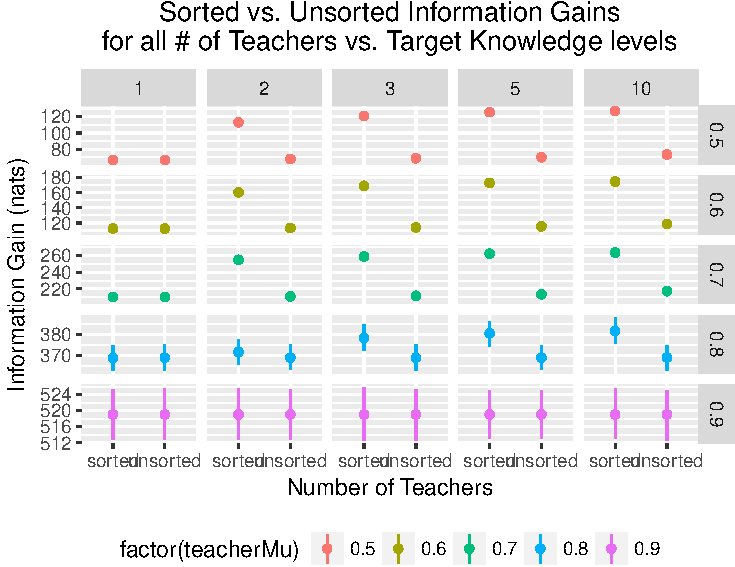
\includegraphics[width=3.25in,height=2.6in]{figs/unnamed-chunk-2-1} \caption[Student information gain, plotted by target concept and number of teachers in the school]{Student information gain, plotted by target concept and number of teachers in the school. Information gain represents the gain when students are sorted into classrooms based on knowledge compared with an unsorted baseline. Error bars show 95\% confidence intervals by non-parametric bootstrap.}\label{fig:unnamed-chunk-21}
\end{figure}
\begin{figure}[t]
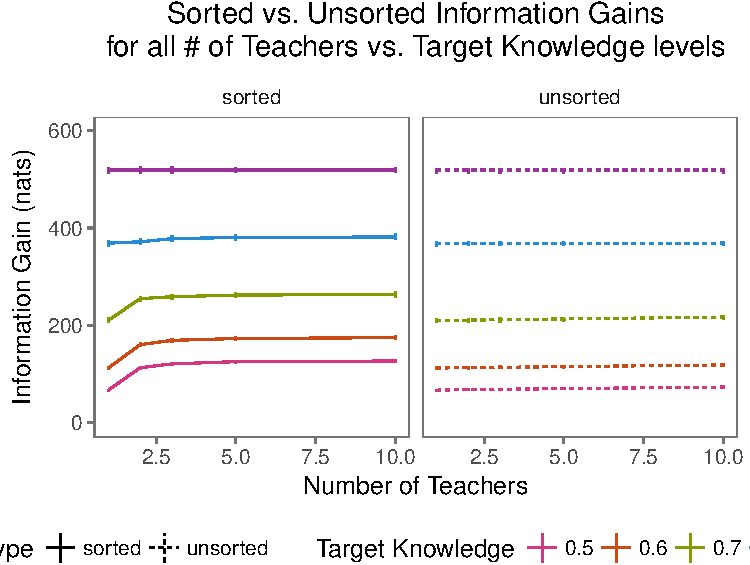
\includegraphics[width=3.25in,height=2.6in]{figs/unnamed-chunk-2-2} \caption[Student information gain, plotted by target concept and number of teachers in the school]{Student information gain, plotted by target concept and number of teachers in the school. Information gain represents the gain when students are sorted into classrooms based on knowledge compared with an unsorted baseline. Error bars show 95\% confidence intervals by non-parametric bootstrap.}\label{fig:unnamed-chunk-22}
\end{figure}
\end{CodeChunk}

In our first analysis, we explored the effects of grouping students by
their \emph{true prior beliefs} (admins with perfect knowledge), so that
teachers can tailor the examples they teach to that particular group.
This analysis is a replication of results reported in Frank (2014) using
the multi-classroom model developed here. We hypothesized that sorting
students by their true beliefs would increase information gain compared
to random classroom assignment. Our baseline for this analysis was the
unsorted information gain under the same parameters. For instance, the
sorted aggregate IG of a school with 5 teachers and a target bias of .6
is compared to the unsorted aggregate IG for a school with 5 teachers
and a target bias of .6 using the same school of students.

Results are shown in Figure 1. Sorted students show greater information
gain than if the same set of students are distributed into unsorted
classrooms. This effect is present for all target concepts but is most
pronounced for less-extreme concepts -- for extreme value concepts
(e.g., a target of .9), almost all students will benefit from seeing the
same examples anyway, rendering sorting irrelevant. Thus, an optimal
school administrator with perfect student knowledge should consistently
opt to sort students into classrooms by their prior beliefs over random
assignment.

\subsection{Simulation 2: Class size}\label{simulation-2-class-size}

\begin{CodeChunk}
\begin{figure}[t]
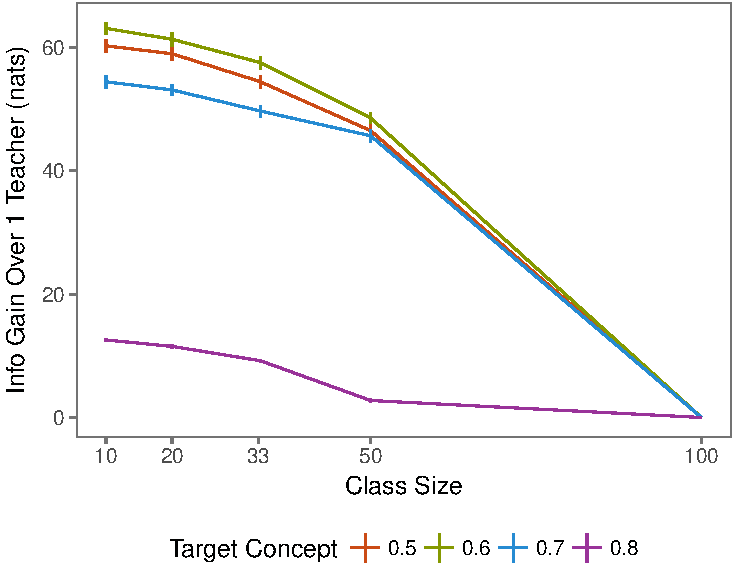
\includegraphics[width=3.25in,height=2.6in]{figs/sim_class_size-1} \caption[Student information gain, plotted by target concept and class size]{Student information gain, plotted by target concept and class size. Information gain represents the gain when students are sorted into classrooms based on knowledge compared with a single-classroom baseline. Error bars show 95\% confidence intervals by non-parametric bootstrap.}\label{fig:sim_class_size}
\end{figure}
\end{CodeChunk}

In our second analysis, again a replication of our prior work, we
explored the effects of adding teachers to the simulated school, leading
to lower class sizes. We hypothesized that increasing the number of
teachers would strictly improve student learning rate (again assuming
perfect knowledge about students): more teachers in a school means that
students are in smaller classes and hence receive better customized sets
of examples from the teacher that appropriately helps students calibrate
their prior beliefs towards the target concept. Our baseline for this
analysis was the sorted information gain under the same target bias
parameters. We observed the predicted pattern (Figure 2), although there
were diminishing returns. After a certain number of teachers, additional
lesson customization becomes less helpful.

\subsection{Analysis 3: Noisy students and
assessments}\label{analysis-3-noisy-students-and-assessments}

In our third analysis, we relax the assumption that teachers have
perfect knowledge about students. In the real world, neither the admin
nor the teacher is an omniscient being that knows the true prior student
belief parameters. Instead, they diagnose student beliefs by
administering assessments (e.g.~placement exams). Using the outcome of
these assessments, school faculty can estimate the existing beliefs that
students hold, and teach to those beliefs.

\subsubsection{Simulation details}\label{simulation-details-1}

\subsubsection{Student noisiness}\label{student-noisiness}

To model these agent behaviors, we assume that the admin and teachers
start with a na"ive, uniform representation of each student (i.e.
\(Beta(1,1)\)) and learn about the student's prior beliefs via the
administration of assessments. In assessments, students are called upon
to demonstrate their knowledge by sampling from their own true
distribution. These samples then serve to update the teacher's estimate
about student knowledge. In this sense, the teachers and administrator
are modeled as a perfect Bayesian agent that updates its beliefs about
student knowledge based on evidence it sees from student performance on
assessments.

For instance, a student may have a true prior belief represented by
\(Beta(9,2)\). When assessed, they are extremely likely to respond with
\(H\) (or \(1\)) to each question on the assessment. If they are asked 6
questions, the most common outcome will be \({H, H, H, H, H, T}\). The
teachers and administrator starts with the naive \(Beta(1,1)\)
representation of the student beliefs, but then updates it for seeing 5
heads and 1 tail in the assessment phase. Their \emph{guessed belief} of
student learning becomes \(Beta(6,2)\) after the Bayesian update. By
construction, our uncertain teachers have very weak and inaccurate
beliefs about student knowledge, captured by the low magnitude of the
initial Beta parameters, and we assume that increasing assessments will
help them improve the accuracy of their representation of student
knowledge.

\paragraph{Effects of sorting in a noisy
setting}\label{effects-of-sorting-in-a-noisy-setting}

\subsubsection{Currency of time}\label{currency-of-time}

We hypothesize that increasing the number of assessments monotonically
improves student learning on average, though with diminishing returns.
As such, simply measuring information gain as the number of assessments
increases is rather trivial. In this simulation, we introduce the
currency of time--each student spends a fixed amount of 12 time steps in
the school system, and any single time step can be devoted to assessing
the student (3 samples from the student's prior distribution about the
learning concept) or a teacher showing the student one piece evidence (a
heads or a tails). By modeling the tradeoff between increasing
assessments and increasing teaching opportunities, we attempt to
identify a tipping point at which giving teachers more opportunities to
show examples outweight the diminishing returns on information gain of
increasing assessments.

\subsubsection{Baseline}\label{baseline}

We have a baseline model that uses a non-inferential admin and teacher.
This admin and teacher does not take their students' prior beliefs into
consideration, and simply selects a set of examples that they believe is
an accurate representation of the target concept. \textbf{TODO:
ELABORATE HERE}

For each trial, we test students in two conditions of faculty knowledge:
omniscient teachers with perfect knowledge vs.~uncertain teachers with
noisy knowledge. The full set of control parameters spans 2 (sorted
vs.~unsorted students) x 5 (target concepts) x 5 (number of teachers) x
13 (number of assessments = 12 - number of teaching periods) = 650
different regimes.

teachers and administrators who have perfect knowledge of students and
sort them into classrooms via this knowledge teachers who have perfect
knowledge, but with students randomly assigned to their classroom
teachers and administrators both have uncertainty about student
knowledge, with administrators sorting students and teachers selecting
examples based on assessment results, and teachers who have uncertainty
about student knowledge and select examples based on assessment results,
with students randomly assigned to their classroom

\begin{CodeChunk}
\begin{figure*}[t]
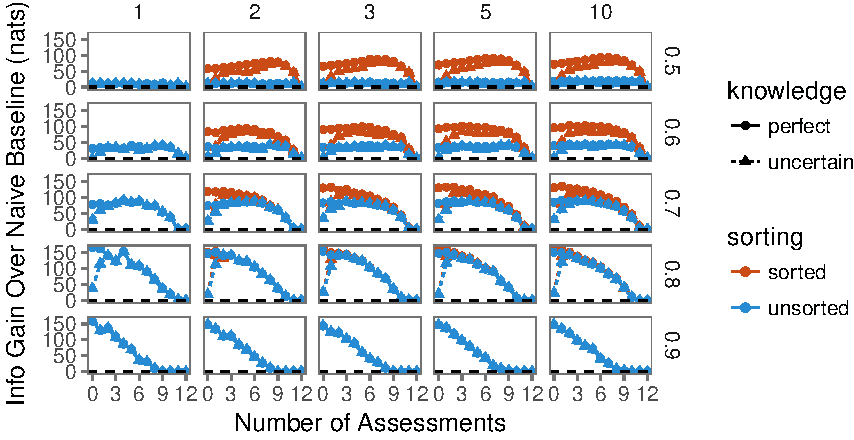
\includegraphics[width=3.25in,height=2.6in]{figs/sim_noisy_students-1} \caption[Information gain plotted by number of assessments (out of 12) for teachers with perfect and uncertain student knowledge]{Information gain plotted by number of assessments (out of 12) for teachers with perfect and uncertain student knowledge. Results shown are for 5 teachers.}\label{fig:sim_noisy_students}
\end{figure*}
\end{CodeChunk}

We hypothesized that with uncertainty about student knowledge, teachers
should perform strictly worse in any given regimes of control parameters
than if they had omniscient, perfect knowledge about the student prior
beliefs. We further hypothesized that there would be a non-linear effect
of number of assessments on information gain. Having too few assessments
would be non-optimal because teachers and administrators cannot
accurately gauge student learning, causing administrators to make more
errors in sorting students by ability level and teachers to select
examples that don't maximize student learning within their classrooms.
Having too many assessments would also be non-optimal because teachers
do not have enough opportunities to precisely teach the examples they
would want. In other words, there are diminishing returns to the number
of assessments performed.

As expected, we found that the uncertain teachers performed strictly
worse than the omniscient teachers when controlling for every other
feature (sorting, target concept, number of teachers, number of
assessments). Furthermore, consistent with Analysis 1, sorting the
students produced greater gains for student learning relative to not
sorting the closer the teacher mu is to 0.5. Even with the uncertainty
in teacher beliefs about student knowledge, students learned more when
the classrooms were sorted by ability than when the teachers had perfect
knowledge in unsorted classrooms. Consistent with Analysis 2, decreasing
class size also improves student learning, though also with diminishing
returns.

Additionally, we found a concave down shape in the student IG based on
number of assessments that is consistent with our non-linearity
hypotheses. Between teacher mus of 0.5 and 0.7, the optimal number of
assessments is greater than 0 and less than 12. As teacher mu approached
0.5, i.e.~as greater variation in student beliefs relative to the true
learning concept increased, the higher the number of optimal number of
assessments. The optimal number of assessments also decreases as the
number of teachers increase. In both cases, it appears that the optimal
number of assessments increases when there exists a possibility of
greater intra-classroom variation on student prior beliefs.

\begin{CodeChunk}

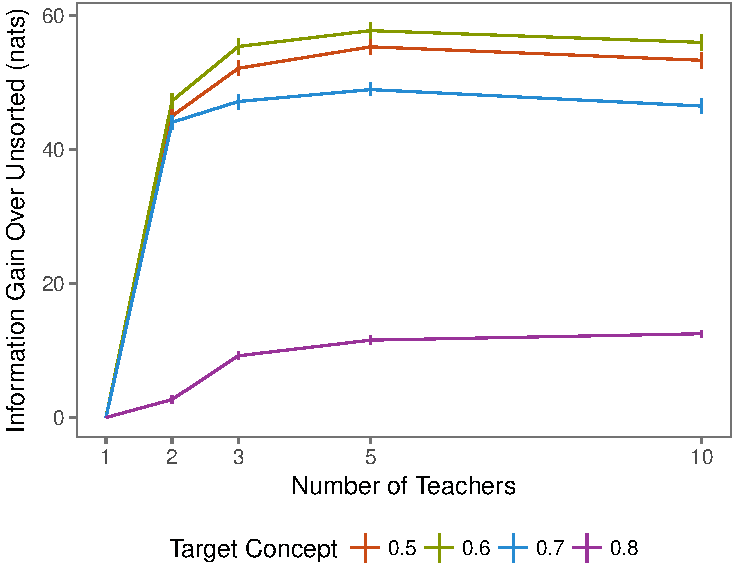
\includegraphics[width=3.25in,height=2.6in]{figs/unnamed-chunk-4-1} 
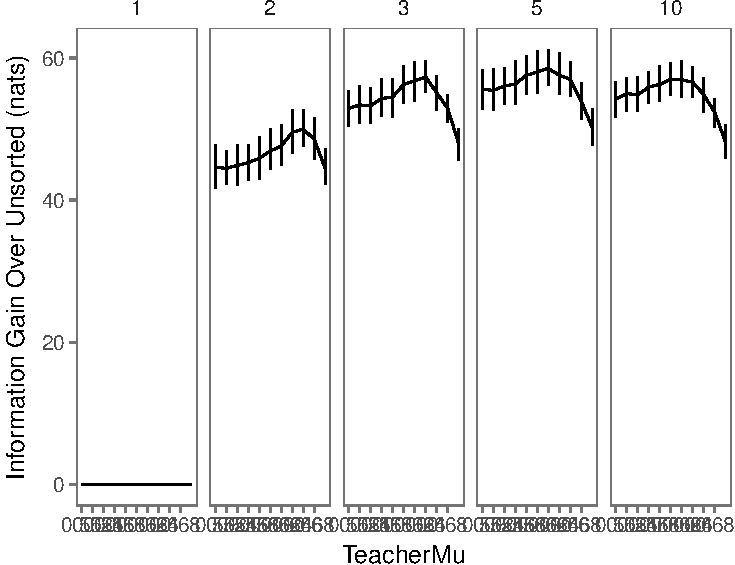
\includegraphics[width=3.25in,height=2.6in]{figs/unnamed-chunk-4-2} \end{CodeChunk}

\begin{CodeChunk}

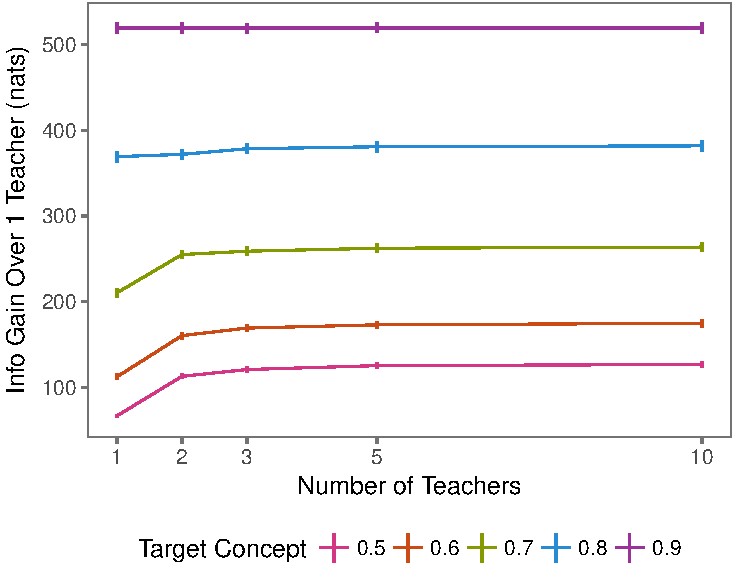
\includegraphics[width=3.25in,height=2.6in]{figs/unnamed-chunk-5-1} \end{CodeChunk}

\begin{CodeChunk}

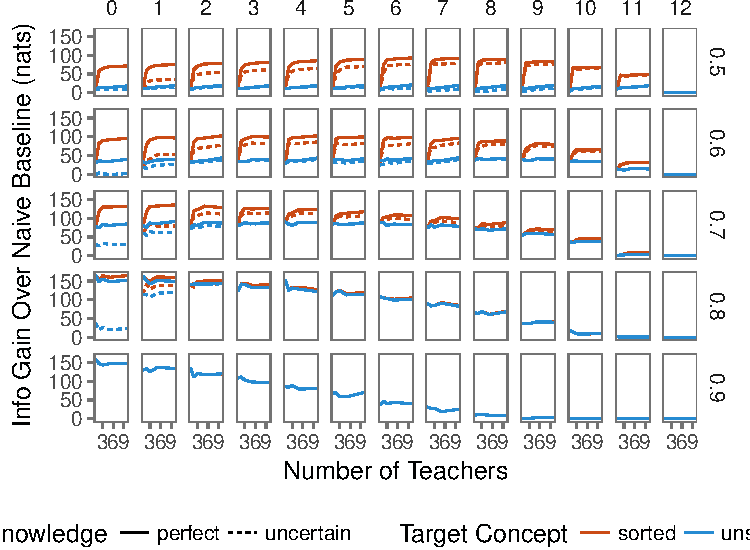
\includegraphics[width=3.25in,height=2.6in]{figs/unnamed-chunk-7-1} \end{CodeChunk}

The admin uses these estimates to sort students into classrooms, and
teachers use these estimates to customize the set of teaching lessons to
a particular student group.

In the simulation, the students have a limited number of learning
opportunities. We found that increasing aggregate IG converges quick
after 10 time steps (noticeable in Figure 5), so we report results with
an arbitrarily chosen 12 time steps. Each assessment or lesson takes 1
time step, and all assessments come before all lessons.

We hypothesized that the noisy students will produce less information
gain than if the faculty had perfect knowledge of student beliefs. We
suspect the school design will differ from the optimal configurations at
two stages: the sorting stage (classrooms will not have maximal
homogeneity), and the teaching stage (the examples selected by any given
teacher will not maximize IG for the students assigned to their class).
Nevertheless, we still believe the improvements to IG by increasing the
number of teachers and reducing class sizes would persist for noisy
students.

We further hypothesized that the optimal use of the allotted time steps
would involve a small or moderate number of assessments and a moderate
to large number of lessons. We thought that a few assessments would get
the estimated beliefs about student knowledge close enough to the
students' true beliefs to minimize sorting errors, leaving teachers with
enough time to teach lessons to move the students' actual beliefs
towards the target concept. Too many assessments would reduce the amount
of time teachers have to teach regardless of how precise their estimates
of student knowledge are; too few assessments would prevent teachers
from selecting helpful examples in their lessons.

Indeed, we found a quadratic shape in the relationship between number of
assessments and aggregate IG. Assessing students helps improve learning
rate by giving teachers better estimates of their beliefs, but they
still need time to subsequently teach towards the target concept.
Additionally, like previous simulations, this effect was most pronounced
in moderate target concepts. These results make intuitive sense.
Teaching concepts where there may be greater variance in student
knowledge relative to each other (e.g.~teaching concepts of .5) demand
more customization in lesson plans with students exhibiting different
levels of mastery.

\subsection{Simulation 4: Pareto frontier with imposed budget
constraints}\label{simulation-4-pareto-frontier-with-imposed-budget-constraints}

\begin{CodeChunk}

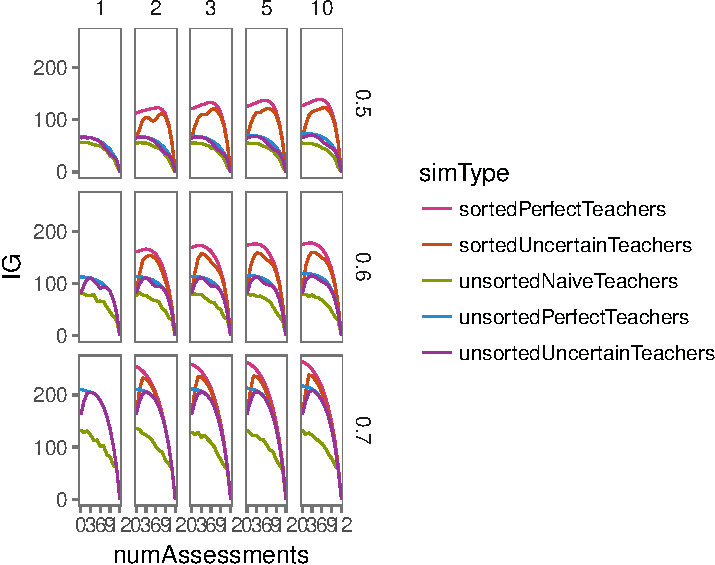
\includegraphics[width=3.25in,height=2.6in]{figs/unnamed-chunk-9-1} \end{CodeChunk}

We hypothesized that for a particular budget constraint and fixed costs
of teachers and assessment, there will be a Pareto frontier of possible
allocations of that budget towards teachers and assessments on which
there will be an optimal allocation that maximizes student learning.
Furthermore, we hypothesized that the individual results about number of
teachers number of assessments would hold within levels of the other.
This is the unification of all previous simulations into one model that
allows us to introduce a real-world constraint of budget.

In this simulation, we test all integer combinations of number of
teachers between 1 and 10 with number of assessments between 0 and 5. We
assigned the cost of each teacher to be CT = \$10 and the cost of each
assessment CA = \$20.

Our baselines were the worst-performing within-target setup. This always
happened to be the 1-teacher 0-assessment setup, which is consistent
with existing education literature, since a single teacher cannot
significantly differentiate learning, and still has a lot of uncertainty
about student beliefs because no assessments are performed.

Our simulated findings support our hypothesis. There is con- siderable
support for an interaction model between teachers, assessments, and the
target bias, F(7, 112) = 48.61, p\textless{}.001. To visualize the
pareto frontier, we draw a heatmap of scores

above baseline along teacher and assessment axes. We con- tinue to see
that the effects continue to be weaker for more extreme learning
concepts, t(294) = -11.09, p\textless{}.001. This result can be seen in
Figure 5.

Since real-world learning concepts are essentially non- negotiable, the
effectiveness of a particular allocation of bud- get should be judged
within-target, i.e.~an optimal setup within the target bias = 0.8 level
should not be penalized for being ineffective in comparison to the
optimal setup for teaching a target bias of 0.5. We normalized the
information gain above baseline within each target bias level. The
results can be seen in 6

Consistent with Simulation 3, increasing the number of assess- ments on
average improves learning rate up until you cannot afford any more
assessments, across all levels of teachers and target biases. Consistent
with Simulation 2, increasing the number of assessments improves
learning rate up until you cannot afford any more assessments, across
all levels of assessments and target biases of 0.5, 0.6, and 0.7.

An interesting result, however, is that having noisy students diminishes
the effectiveness of increasing the number of teach- ers at certain a
target bias of 0.8. While we aren't sure of the specific mechanism by
which this happens, we suspect that having more teachers introduces
additional risk of wrongly sorting students' prior beliefs, which would
increase the het- erogeneity of classrooms. Since a target belief of 0.8
is a possible target belief to show precisely with 5 examples (the basis
of our simulations) but also extreme enough that most students's prior
belief will fall on one side of that target, in- creasing the number of
teachers might actually reduce the effectiveness of the teacher's choice
of examples. A novel finding that emerged not described in existing
educa- tion literature is that there are different patterns of
optimality along the pareto frontiers. As the extremity of the target
bias moves from 0.5 to 0.7, we see that the IG-optimal allocation of
budget shifts from about 5-6 teachers and 2 assessments towards more
assessments at the expense of the number of teachers.

\section{Discussion}\label{discussion}

Summary

In our simulations, we refer to the entire group of students as a
``school,'' broken into ``classrooms,'' and students are given
``assessments'' and ``lessons.'' These mappings are inexact, however,
and the analogical correspondence can be made at a lower level. For
example, the same set of ideas could be applied \emph{within a
classroom}, for example to the decision whether to split the class into
smaller groups and divide the teachers time amongst supervising them.
And similarly, what we describe ``assessments'' and ``lessons'' could be
either multi-item tests and then several days of instruction or -- again
at a more micro scale -- a single question posed to the class followed
by several pieces of related content within a single class session. Our
goal is to elucidate general principles that govern the process of
teaching rather than to claim a correspondence with specific phenomena
or teaching methodology.

Overall, we were able to replicate many real-world findings from
education literature. We found that sorting students into ability level
classrooms, increasing assessment, and decreasing class size all
increase information gain.

One of the more interesting findings was the influence of the target
bias on the effects we were finding. Based on our results, target bias
significantly moderates each of the effects we found. When teaching an
extremely difficult (or easy, given symmetry) learning concept such that
all student prior beliefs are on one side of the concept, the payoffs to
information gain that sorting, class sizes, and assessment have diminish
because regardless of the level of noise, teachers have relative
certainty about the students' relative level of understanding.
Similarly, target biases that are very close to central (around 0.5)
have a lot to gain from diminishing noise in the system.

Finally, we found that the relative effectiveness of number of teachers
and and the number of assessments varies depend- ing on the target
learning concept. We saw that the most optimal distribution of budget on
the pareto frontier shifted towards reducing student noise when the
target bias was more extreme--this seemed consistent with intuition,
since having more teachers doesn't allow them to better select examples
if the administrator produces greater sorting errors, resulting in
heterogeneous classrooms where each teacher has less cer- tainty about
whether their examples will be useful for any particular student or not.

While a lot of aspects of school learning (peer effects, social
dynamics, etc.) are not built into our model and would be difficult to
capture algorithmically, we believe that there is a lot to be gained
from simulating classroom dynamics. Using stochastic modeling is
particularly useful when exploring the effectiveness of education policy
measures for a handful of reasons. Fundamentally, the merits of
stochastic modeling arise from the use of synthetic data. Since the
studies are computer-simulated, there are no human subjects in the stud-
ies, and all of the data is synthetic. This allows researchers to take
greater liberties in experimental design because there are no ethical
concerns. For instance, we can execute a sim- ulation that will
intentionally misclassify synthetic students into classrooms that are
not appropriate for their achievement level to understand the negative
impact doing so has on both the misclassified student and his peers.
Such a study would not be ethically permissible in an actual school.

Furthermore, no two schools are the same, and the use of mod- eling and
synthetic data enables rapid iteration over different simulated schools
with different simulated students. We can quickly test whether the
purported benefit to student learning of various education interventions
holds with, for example, a limited budget, or highly varied student
achievement levels, or immensely large class sizes. There is also no
risk of student subject attrition that may jeopardize real-world school
studies; synthetic students do not exhibit unpredictable absenteeism,
transfer schools, take sick days, etc. As such, we can cus- tomize our
interventions based on school parameters, validate the robustness of our
results, and better infer generalized find- ings about education policy
without incurring astronomical experimental monetary costs nor require
lengthy longitudinal study. With a complete stochastic model, we can
quickly scale the number of hypotheses we test and the variety of
schools we test them on. Our series of simulations are designed to
replicate real-world results from education literature in a
quantitative, simulated fashion. The first few simulations looked at a
lot of existing educational theory in isolation, while our final
simulation attempts to unify these different design aspects of a school
system into a more holistic view. We found that increasing the number of
teachers (and thus decreasing class size) and increasing the amount of
assessment to improve precision about student beliefs increases student
learning, as predicted in real-world school studies.

Importantly, we were able to generate pareto frontiers allocating a
fixed shared resource of budget into the dimensions of teachers and
sorting. The ability to make sense of the tradeoffs that school
administrators and policymakers need to make when designing their
schools can help improve education. This would be particularly impactful
in communities of low socioeconomic status where academic achievement
tends to be lower because budgets are particularly constrained and
attracting teaching staff is difficult.

Some of the limitations of the present work is in the assump- tions that
we make to build our model. Most obvious is the simplicity of the
learning task we described during the intro- duction. Most real-world
learning tasks are more complicated and may have multiple objectives.
Furthermore learning in the real-world is affected by a lot of more
abstract facets: peer learning and social environment, parenting styles,
stereotype threat, among other things. These are not captured in the
model, and would be difficult to capture in any model. The agnostic
prior beliefs we 1) use for teachers to generate examples from; 2)
generate student prior beliefs from; and 3) create target bias
distributions with are all uniform distri- butions. These are not
necessarily the case. Respectively, 1) teachers may have prior beliefs
about which examples are more effective, akin to pedagogical knowledge
or pedagogical content knowledge (Cochran, 1991); 2) students may tend
towards certain common prior beliefs/misconceptions about a particular
learning concept; 3) more extreme learning concepts may be more rare,
and thus the admin should weight more heavily the pareto frontier of
moderate target bias values.

\section{Acknowledgements}\label{acknowledgements}

This work supported by NSF BCS \#1456077.

\section{References}\label{references}

\setlength{\parindent}{-0.1in} \setlength{\leftskip}{0.125in} \noindent

\hypertarget{refs}{}
\hypertarget{ref-cohen1982}{}
Cohen, P. A., Kulik, J. A., \& Kulik, C.-L. C. (1982). Educational
outcomes of tutoring: A meta-analysis of findings. \emph{American
Educational Research Journal}, \emph{19}(2), 237--248.

\hypertarget{ref-cover2012}{}
Cover, T. M., \& Thomas, J. A. (2012). \emph{Elements of information
theory}. John Wiley \& Sons.

\hypertarget{ref-frank2014}{}
Frank, M. C. (2014). Modeling the dynamics of classroom education using
teaching games. In \emph{CogSci}.

\hypertarget{ref-frank2012}{}
Frank, M. C., \& Goodman, N. D. (2012). Predicting pragmatic reasoning
in language games. \emph{Science}, \emph{336}(6084), 998--998.

\hypertarget{ref-fuchs1986}{}
Fuchs, L. S., \& Fuchs, D. (1986). Effects of systematic formative
evaluation: A meta-analysis. \emph{Exceptional Children}.

\hypertarget{ref-glass1979}{}
Glass, G. V., \& Smith, M. L. (1979). Meta-analysis of research on class
size and achievement. \emph{Educational Evaluation and Policy Analysis},
\emph{1}(1), 2--16.

\hypertarget{ref-goodman2016}{}
Goodman, N. D., \& Frank, M. C. (2016). Pragmatic language
interpretation as probabilistic inference. \emph{Trends in Cognitive
Sciences}, \emph{20}(11), 818--829.

\hypertarget{ref-goodman2017}{}
Goodman, N. D., \& Stuhlmüller, A. (n.d.). The design and implementation
of probabilistic programming languages. Retrieved 2017, from
\url{http://dippl.org}

\hypertarget{ref-sadler1989}{}
Sadler, D. R. (1989). Formative assessment and the design of
instructional systems. \emph{Instructional Science}, \emph{18}(2),
119--144.

\hypertarget{ref-slavin1987}{}
Slavin, R. E. (1987). Ability grouping and student achievement in
elementary schools: A best-evidence synthesis. \emph{Review of
Educational Research}, \emph{57}(3), 293--336.

\hypertarget{ref-slavin1989}{}
Slavin, R. E. (1989). Class size and student achievement: Small effects
of small classes. \emph{Educational Psychologist}, \emph{24}(1),
99--110.

\hypertarget{ref-slavin1990}{}
Slavin, R. E. (1990). Achievement effects of ability grouping in
secondary schools: A best-evidence synthesis. \emph{Review of
Educational Research}, \emph{60}(3), 471--499.

\hypertarget{ref-tomlinson1999}{}
Tomlinson, C. A. (1999). \emph{The differentiated classroom: Responding
to the needs of all learners}. Association for Supervision \& Curriculum
Development.

\end{document}
